\documentclass[../main.tex]{subfiles}
\graphicspath{{\subfix{../IMAGES/}}}

\begin{document}
\localtableofcontents
\subsection{Classification des méthodes de résolution}
On peut séparer les méthodes en trois parties distinctes : \\
\begin{itemize}
    \item Forme forte : la fonctionnelle doit être définit en chaque point de l'espace (méthode des différences finies) $D(u) = f$\\
    \item Forme intégrale : la fonctionnelle n'est pas forcément valable en chaque point $\int_\omega v^T [D(u)-f]d\omega = 0 \forall v$ (méthode des résidus pondérés\\
    \item Forme faible : On intègre ici par partie $\int_\omega ([D'(v)]^T D'(u) - v^T f)d\omega + TB = 0 \forall v$ (méthode de Galerkin/éléments finis)\\
\end{itemize}

Par exemple, équilibre de la barre : \\
Formulation forte : $-EA \left( \frac{d^2 u}{dx^2} \right) = a$ dans $]0,l[$, $u\in C^2(]0,l[)$, $q\in L^2 (]0,l[)$\\

On appelle \textbf{condition aux limites essentielle} celles qui influent directement la solution (ex : $u(0)=0$)\\
On appelle \textbf{condition aux limites naturelle} celles qui touchent à la dérivée de celle-ci (ex : $EA \frac{du}{dx} = P$)\\

La formulation intégrale du problème est alors : $\int_0^l [EA(\frac{d^2u}{dx^2})+q]\delta u dx = 0$ $\forall \delta u$ \warning $\delta u$ possède un caractère arbitraire.\\

Ensuite, en appliquant les conditions aux limites essentielle au déplacement virtuel pour obtenir un \textbf{déplacement virtuel cinématiquement admissible}. En utilisant une intégration par partie, on obtient la formulation faible du problème :\\
$u \in U : \int_0^l EA 8\frac{du}{dx})(\frac{d\delta u}{dx}) dx = P\delta u(l) + \int_0^l q \delta udx \forall \delta u \in V$\\

Où U et V sont tels que : \begin{itemize}
    \item $U= \{ u(x) | u(x) \in H^1(]0,l[)$; $u(0)=0\}$\\
    \item $V = \{ \delta u(x) | \delta u(x) \in H^1(]0,l[); \delta u(0) =0\}$\\
\end{itemize}

\subsection{Définition des classes de fonctions}
\begin{itemize}
    \item Classe des fonctions à dérivées continues d'ordre k : $C^k(]0,l[) = \{u(x), \cdot, \frac{d^ku}{dx^k}$ continues $|$ $|u|_k < \infty \}$\\
    \item Norme maximale bornée : $|u|_k = \max_{0\leq q\leq l} (|u| + \cdot + |\frac{d^ku}{dx^k}|)$\\
    \item Régularité : $|u|_0 \leq |u|_1 \leq \cdot$, $\cdot C^2 \subset C^1 \subset C^0$\\
    \item Classe des fonctions à dérivées de carrées sommables d'ordre k (espace de Sobolev/Hilbert) : $H^k (]0,l[) = \{ u(x)| \Vert u \Vert_k < \infty \}$\\
    \item Norme hilbertienne : $\Vert u\Vert_k = \{ \int_0^l [u^2 + (\frac{du}{dx})^2+ \cdot + (\frac{d^k u}{dx^k})^2]dx \}^{\frac{1}{2}}$\\
    \item Régularité : $\Vert u \Vert_0 \leq \Vert u \Vert_1 \leq \cdot$ $\cdot H^1 \subset H_0$\\
    \item Classe des carrés sommables : espace de Sobolev d'ordre 0 $L^2 = H^0$\\
\end{itemize}

Comparaison des classes de fonctions : \begin{itemize}
    \item Inclusion des classes de fonctions : $C^k \subset H^k$ $(k\geq 0)$\\
    \item Théorème d'injection de Sobolev (n dimension du problème) $C^k \subset H^k \subset C^h$ $(k-h > n/2; k,h>0)$\\
\end{itemize}

\subsection{Formulation faible approchée/méthode de Galerkin}
\begin{itemize}
    \item Approximation des déplacements axiaux réel et virtuel \begin{equation}
        \begin{split}
            u \simeq u^h \in U^h \subset U\\
            \delta u \simeq \delta u^h \in V^h \subset V
        \end{split}
    \end{equation}
    \item Forme faible approchée : \begin{equation}
        u^h \in U^h : \int_0^l EA (\frac{du^h}{dx})(\frac{d\delta u^h}{dx})dx = P \delta u^h(l) + \int_0^l q \delta u^h dx
    \end{equation}
    \item Choix de n fonctions de forée linéairement indépendantes, constituant une base du sous-espace $U^h$ de dimension n\\
\end{itemize}

\quad \underline{Approximation de Galerkin :}\\
\begin{equation}
    u^h(x) = \sum_{i=1}^n \alpha_i h_i(x) = \mathbf{H}(x) \mathbf{\alpha}
\end{equation}

Avec $\mathbf{H}$ une matrice 1xn des \textbf{fonctions de forme} et $\mathbf{\alpha}$ un vecteur nx1 des inconnues\\

De même pour $\delta u^h(x) = \mathbf{H}(x) \delta \mathbf{\alpha}$

Les \textbf{fonctions $h_i(x)$ définies globalement} sur le domaine [0,l] et \textbf{respectant les conditions aux limites essentielles}.\\

\quad \underline{Détail de la méthode :}\\
\begin{equation}
    \begin{split}
        \int_0^l EA [\frac{d \mathbf{H}\delta \mathbf{\alpha}}{dx} \frac{d \mathbf{H} \mathbf{\alpha}}{dx}]dx = [\mathbf{H}(l) \delta \mathbf{\alpha} P] + \int_0^l \mathbf{H} \delta \mathbf{\alpha}dx\\
        \Rightarrow \delta \mathbf{\alpha}^T [\int_0^l EA (\frac{d \mathbf{H}^T}{dx})(\frac{d \mathbf{H}}{dx})dx \mathbf{\alpha}- \mathbf{H}^T(l)P + \int_0^l \mathbf{H}^Tqdx] = 0\\
        \Rightarrow \delta \mathbf{\alpha}^T (\mathbf{K} \mathbf{\alpha}-\mathbf{r})=0 \forall \delta \mathbf{\alpha}
    \end{split}
\end{equation}

On obtient dès lors la \textbf{forme faible discrète} : \begin{equation}
    \mathbf{K} \mathbf{\alpha} = \mathbf{r}
\end{equation}

\begin{itemize}
    \item $\mathbf{K} = \int_0^l EA (\frac{d \mathbf{H}^T}{dx})(\frac{d\mathbf{H}}{dx})dx$ la \textbf{matrice de rigidité}\\
    \item $\mathbf{r} = \mathbf{H}^T(l)P + \int_0^l \mathbf{H}^T qdx$, le \textbf{vecteur des forces appliquées}\\
    \item $\mathbf{B} = \frac{d\mathbf{H}}{dx}$ la \textbf{matrice-déformation} ou de passage des déplacements aux déformations\\
\end{itemize}

\subsubsection{Avantages et Inconvénients}
\begin{itemize}
    \item Avantages : \begin{itemize}
        \item même approximation pour $u^h$ et $\delta u^h$ : construction d'un seul sous-espace $U^h$ et d'un seul ensemble de fonctions $h_i(x)$\\
        \item meilleure approximation possible de $u^h$ dans le sous-espace $U^h$\\
    \end{itemize}
    \item Inconvénients : \begin{itemize}
        \item Aucune information pour la construction des fonctions de forme $h_i(x)$\\
        \item Difficultés à trouver des fonctions $h_i(x)$ globales satisfaisant les conditions aux limites essentielles\\
        \item $\alpha_i$ sans interprétation physique\\
    \end{itemize}
\end{itemize}

Accroissement de la précision globale avec le nombre n de termes dans l'approximation $u^h$. Solution exacte en $x=0$ (condition aux limites essentielle vérifiée par l'approximation. Condition aux limites naturelle approchée en $x=l$ mais, approximation améliorée avec le nombre n de termes.\\

\subsection{Méthode des éléments finis : approche globale}
Éléments finis se touchent aux points nodaux. Ici, on discrétise en éléments finis à deux noeuds. \\
En 2D, m éléments finis correspondent à p+1 point nodaux.\\

\begin{equation}
    \begin{gathered}
        u^h(x) = H(x) q\\
        \partial u^h(x) = H(x) \partial q\\
    \end{gathered}
\end{equation}
Où : \begin{itemize}
    \item H est la matrice (1xp) : \textbf{fonctions de forme nodales}\\
    \item q est le vecteur (px1) : \textbf{déplacements nodaux}\\
\end{itemize}

Les fonctions $h_i(x)$ sont à \textbf{support compact} : nulle partout sauf sur un segment de deux éléments finis $\Omega$\\

\warning Respect nécessaire de la condition aux limites essentielle par la fonction $h_0$\\

Quelques conditions sur les fonctions $h_i$ : \begin{itemize}
    \item Critère de complétude : fonctions $h_i$ affines sur les éléments; constituant une base complète permettant la représentation des états de déformation constante et les déplacements rigides\\
    \item Critère de différentiabilité : les fonctions $h_i$ doivent être suffisamment \textbf{régulières} à l'intérieur des éléments pour assurer $u^h \in U^h$\\
    \item Critère de continuité : les fonctions $h_i$ doivent être continues aux interfaces des éléments\\
\end{itemize}

Dans cette méthodes, les inconnues ont une représentation physique : $h_i(x_j) = \partial_{ij}$ $\Rightarrow u^h(x_j) = q_j$\\
Les $q_j$ sont donc les déplacements du point j\\

De la même manière que Galerkin, on a le système : \begin{equation}\begin{gathered}
    Kq = r\\
    k_{ij} = \int_0^l EA \frac{dh_i}{dx} \frac{dh_j}{dx}dx\\
    r_i = h_i(l)P + \int_0^l h_iqdx\\
    \end{gathered}
\end{equation}
De manière générale, la matrice K est éparse (tri-diagonale en général).\\

\subsubsection{Avantages et inconvénients}
\begin{itemize}
    \item Avantages : \begin{itemize}
        \item Systématisation du processus : approximation sous la forme de polynômes de faible degré continus par morceaux\\
        \item Fonctions de forme à support compact : matrice de rigidité peu dense, condition aux limites essentielle satisfait par une fonction\\
        \item Interprétation physique des éléments\\
    \end{itemize}
    \item Inconvénients :\begin{itemize}
        \item Prise en compte limitée de la compacité des fonctions de forme nodales\\
        \item Pas de mise à profit de l'additivité de l'intégration\\
    \end{itemize}
\end{itemize}

\subsection{Méthode des éléments finis : approche locale}
On sélectionne un éléments générique à deux noeuds $^e\Omega$ sur lequel on retrouve deux fonctions de base : ${}^eh_i(x)$ que l'on pourra généraliser au système entier.\\

\begin{itemize}
    \item ${}^eu^h(x) = {}^eH(x) {}^eq$ : ${}^ep$ le nombre de noeuds de l'élément ${}^e\Omega$\\
    \item ${}^eH$ la matrice $(1x {}^ep)$ des fonctions de base\\
    \item ${}^eq$ le vecteur $({}^epx1)$ des déplacements nodaux de l'élément 
\end{itemize}

\quad \underline{Localisation des déplacements nodaux :}\\
\begin{equation}
    {}^eq = {}^eLq
\end{equation}
p : nombre total de noeuds (point nodal 0 compris)\\
${}^eL$ est la matrice $({}^epxp)$ booléenne de localisation.\\
Elle identifie l'emplacement d'un élément finis dans le système.\\

Les mêmes critères s'appliquent sur les fonctions $h_i$ que pour l'approche globale.\\

On a également les critères de continuité restreinte : ${}^eh_i(x_j) = \partial_{ij}$\\
Et de déplacement rigide : $\sum_{i=1}^p {}^eh_i(x)=1$\\

\quad \underline{Assemblage des grandeurs élémentaires :}\\
\begin{equation}
\begin{gathered}
    \sum_{e=1}^m ( \int_{{}^e\Omega} {}^eE {}^eA \frac{d {}^eu^h}{dx} \frac{d {}^e\partial u^h}{dx}dx - P {}^e\partial u^h(l) \partial_{em} - \int_{{}^e\Omega} {}^eq {}^e\partial u^hdx) = 0\\
    Kq = r\\
    K = \sum_{e=1}{}^m {}^eL^T {}^eK {}^eL = A_{e=1}^m {}^eK\\
    r = \sum_{e=1}^m {}^eL^T {}^er = A_{e=1}^m {}^er\\
\end{gathered}
\end{equation}
Avec A l'opérateur d'assemblage.\\

La matrice de rigidité globale se crée en mettant sur la diagonale les sous-matrices ${}^eK$ et en sommant les termes communs.\\

Soit $\xi$ la coordonnée naturelle ou intrinsèque dans $^e\Omega$.\begin{equation}
    \xi = \frac{1}{{}^el}(2x-x_i-x_{i+1})
\end{equation}

Les fonctions de base sont ainsi définies comme : \begin{itemize}
    \item ${}^eh_1 = \frac{1}{2}(1-\xi)$\\
    \item ${}^eh_2 = \frac{1}{2}(1+\xi)$\\
\end{itemize}

Dans le cas de la barre en traction : \begin{itemize}
    \item ${}^ek_{11} = \frac{{}^eE {}^eA}{{}^el}$\\
    \item ${}^ek_{12} = {}^ek_{21} = -\frac{{}^eE {}^eA}{{}^el}$\\
\end{itemize}
Ce qui forme une matrice singulière. \\
\begin{equation}
    K = \begin{pmatrix}
        k_{11} & k_{12} &\\
        k_{21} & k_{22} = {}^1k_{22} + {}^2k_{22} & k_{33}\\
        \dots\\
    \end{pmatrix}
\end{equation}

Pour prendre en compte la condition aux limites essentielle en $x=0$, on pose $q_1=0$ et on retire donc la première ligne de la matrice.\\

\subsubsection{Convergence des modèles}
On définit les normes de l'erreur comme : \begin{equation}
    \lvert \lvert e^h\rvert\rvert_i = \int_0^l (e^h)^2+\sum_{p=1}^i (\frac{d^i e^h}{d (e^h)^i})^2 dx
\end{equation}

On peut dès lors faire une estimation asymptotique de l'erreur : \begin{equation}
    \lvert \lvert e^h\rvert \rvert_k \leq C_k h^p
\end{equation}
Avec : \begin{itemize}
    \item $C_k$ : le facteur de convergence\\
    \item $p$ : le taux de convergence $(p=m+1-k)$\\
    \item $m$ : le degré du polynôme complet des fonctions de base\\
    \item $h$ : longueur caractéristique du réseau ($h = \max {}^el$)\\
    \item $k$ : type de norme\\
\end{itemize}

\subsection{Généralisation aux problèmes unidimensionnels}
On désire un développement d'éléments finis d'ordre supérieur.\\

On ajoute alors des noeuds interne sans rôle de connexion. Ils servent uniquement à la définition des fonctions. Ils doivent être également espacés dans l'espace pour simplifier des calculs.\\

On utilise les polynômes de Lagrange pour déterminer les fonctions de base : \begin{equation}
    {}^eh_i(\xi) = \Pi_{p=1, p\neq 1}^{k+1} \frac{\xi-\xi_p}{\xi_i-\xi_p}
\end{equation}

Ainsi, pour des éléments quadratique (k=2), on a :\begin{itemize}
    \item ${}^eh_1(\xi) = \frac{1}{2}\xi(\xi-1)$\\
    \item ${}^eh_2(\xi) = \frac{1}{2}\xi(\xi+1)$\\
    \item ${}^eh_3(\xi) = 1-\xi^2$\\
\end{itemize}

\warning On pose pour toutes les fonctions de base ${}^eh_i =\begin{cases}
    0 & \forall x\neq x_i\\
    1\\
\end{cases}$\\

\subsubsection{Intégration numérique de Gauss-Legendre}
\begin{equation}
    \int_{-1}^1 pd\xi \simeq \sum_{i=1}^r p\lvert_{\xi = \xi_i}\omega_i
\end{equation}
Où : \begin{itemize}
    \item $\xi_i$ : l'abscisse du point d'intégration i\\
    \item $\omega_i$ : coefficient de pondération du point i\\
\end{itemize}

\warning Avec r points de Gauss, l'intégration est exacte d'un polynôme de degré $2r-1$\\

\subsubsection{Assemblage des matrices}
Comme les indexes réelles et ceux utilisés dans l'élément finis de référence ne sont pas les mêmes (dans l'élément, 1 et 2 sont les points aux extrémités puis 3,4,$\dots$ sont les points entre, alors que dans le système globale on décompte de gauche à droite), il faut inverser des lignes et colonnes des matrices de référence. Par exemple, pour une méthode des éléments finis quadratique, on doit échanger la ligne deux avec la troisième, de même pour les colonnes.\\

\subsection{Insertion de discontinuités}
On pose plusieurs discontinuités : \begin{itemize}
    \item changement de E en $x=x_1$\\
    \item changement de $q$ en $x=x_2$\\
    \item ajout d'une force ponctuelle $Q$ en $x=x_3$\\
    \item modification des conditions aux limites : \begin{itemize}
        \item condition essentielle $x=x_0=0$, $u(0) = \hat{u}$\\
        \item condition naturelle $x=x_4 = l$, $EA \frac{du}{dx}\lvert_{x=l}= -ru(l)+P$ (ressort et charge ponctuelle)\\
    \end{itemize}
\end{itemize}

\begin{figure}[hbt!]
    \centering
    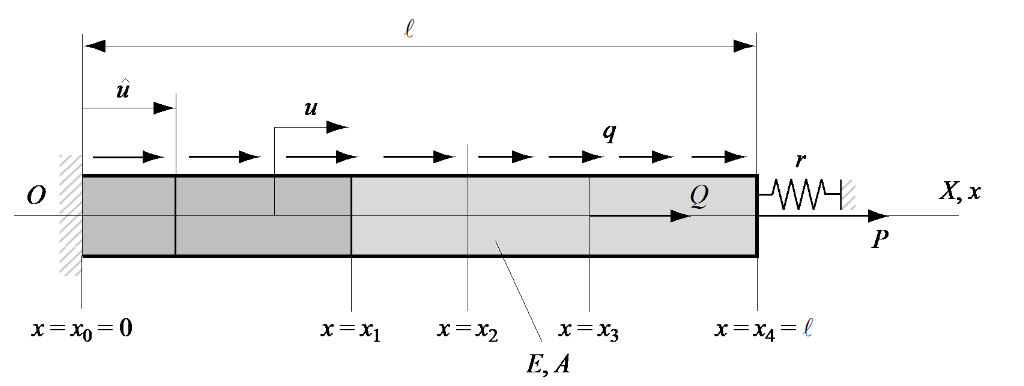
\includegraphics[width=.7\textwidth]{IMAGES/elementfinis/ef1.png}
\end{figure}

On a donc l'équation différentielle : $-\frac{dEA}{dx}(\frac{du}{dx}) + \rho u = q$ avec $\rho$ le facteur de proportionnalité.\\
Pour la forme forte du problème, on a les \textbf{équations de continuité en déplacement :} \begin{itemize}
    \item $\lim_{x\rightarrow x_1^+} u(x) = \lim_{x\rightarrow x_1^-} u(x)$\\
    \item $\lim_{x\rightarrow x_2^+} u(x) = \lim_{x\rightarrow x_2^-} u(x)$\\
    \item $\lim_{x\rightarrow x_3^+} u(x) = \lim_{x\rightarrow x_3^-} u(x)$\\
\end{itemize}

Les \textbf{équations de continuité en flux} : \begin{itemize}
    \item $\lim_{x\rightarrow x_1^+} E(x) \frac{du(x)}{dx} - \lim_{x\rightarrow x_1^-} E(x) \frac{du(x)}{dx} = 0$\\
    \item $\lim_{x\rightarrow x_2^+} E(x) \frac{du(x)}{dx} - \lim_{x\rightarrow x_2^-} E(x) \frac{du(x)}{dx} = 0$\\
    \item $\lim_{x\rightarrow x_3^+} E(x) \frac{du(x)}{dx} - \lim_{x\rightarrow x_3^-} E(x) \frac{du(x)}{dx} = -\frac{Q}{A}$\\
\end{itemize}

La forme intégrale partielle vaut : \begin{equation}\begin{gathered}
    \int_{x_{j-1}}^{x_j} [-\frac{dEA}{dx}(\frac{du}{dx}) + \rho u-q]\delta u dx \neq 0\\
    = \int_{I_j} R\delta u dx = \int_{x_{j-1}}^{x_j} EA \frac{du}{dx} \frac{d\delta u}{dx} + \rho u dx - [EA \frac{du}{dx} \delta u]_{x_{j-1}}^{x_j} - \int_{x_{j-1}}^{x_j} q\delta udx\\
    \Rightarrow \sum_{j=1}^4 \int_{I_j} R\delta udx = 0 \forall \delta u\\
    \end{gathered}
\end{equation}

En appliquant les conditions aux limites dans le cas présent, on obtient : \begin{equation}
    \int_0^l EA \frac{du}{dx} \frac{d\delta u}{dx} + \rho u \delta u dx - Q \delta u(x_3) + (ru(l)-P)\delta u(l) = \int_0^l q \delta u dx 
\end{equation}
Avec \begin{itemize}
    \item $U = \{u(x) \lvert u(x) \in H^1(]0,l[); u(0)=\hat{u}\}$\\
    \item $V = \{\delta u(x) \lvert \delta u(x) \in H^1(]0,l[); \delta u(0)=0\}$\\
\end{itemize}

\subsubsection{Conditions aux limites non homogènes de Dirichlet}
On a maintenant $u(0) = \hat{u}_0$ et $u(l) = \hat{u}_l$. On enlève également le terme $ru$.\\
Alors $\delta u(0) = \delta u(l) = 0$ et: \begin{itemize}
    \item $U = \{u(x) \lvert u(x) \in H^1(]0,l[); u(0)=\hat{u}_0; u(l) = \hat{u}_l\}$\\
    \item $V = \{\delta u(x) \lvert \delta u(x) \in H^1(]0,l[); \delta u(0) = \delta u(l) =0\}$\\
\end{itemize}

\subsubsection{Conditions aux limites non homogènes de Neumann}
On a : \begin{itemize}
    \item $EA \frac{du}{dx}\lvert_{x=0} = P_0$\\
    \item $EA \frac{du}{dx}\lvert_{x=l} = P_l$\\
\end{itemize}
Ici non plus, pas de $ru$.\\
Alors : $U=V = \{w(x) \lvert w(x) \in H^1(]0,l[)\}$\\

\quad \underline{Cas spécial :} \textbf{$\rho=0$}\\
Alors la solution est possible à une constante près ! En effet, comme dans les termes dans les intégrales sont uniquement des dérivées, alors $u$ et $u+d$ donnent la même solution.\\

On a dès lors l'équivalence : \begin{equation}
    \begin{gathered}
        \int_0^l EA \frac{du}{dx} \frac{d\delta u}{dx}dx = \int_0^l q \delta u dx + Q \delta u(x_3) - P_0 \delta u(0) + P_l \delta u(l)\\
        = \int_0^l q(\delta u + d) dx + Q(\delta u(x_3) + d) - P_0(\delta u(0) + d) + P_l(\delta u(l) + d) \\
        \Rightarrow \int_0^l qdx + Q - P_0 + P_l = 0\\
    \end{gathered}
\end{equation}

\subsubsection{Méthode de Galerkin}
On pose les points nodaux aux discontinuités pour convenir au critère de différentiabilié.\\

En règle général, on met tous les termes contenant du $\alpha$ et $\delta \alpha$ à gauche de l'équation et les termes contenant au plus du $\delta \alpha$ à droite de l'équation.\\

\subsubsection{Méthode des éléments finis}
En règle général, on met tous les termes contenant du $q$ et $\delta q$ à gauche de l'équation et les termes contenant au plus du $\delta q$ à droite de l'équation.\\
On approxime également $\hat{q} = q_1 = H()q = u^h(0) \simeq u(0) = \hat{u}$\\

Ici : \begin{itemize}
    \item $K = \int_0^l EA \frac{dH^T}{dx} \frac{dH}{dx} + \rho H^T H dx + r H^T(l) H(l)$\\
    \item $r = \int_0^l H^T qdx + H^T(x_3) Q + H^T(l)P$\\
    \item $Kq = r$\\
\end{itemize}

\warning Comme $u(0) \neq 0$ mais $\delta u(0) = 0$, on peut supprimer la ligne correspondante (ici 1) mais pas la colonne! Pour la supprimer également, on intègre simplement son influence dans le vecteur $r$.\\

Dans notre cas, ${}^eK$ est définie strictement positive ($\lambda$>0).

\subsection{Formulation intégrale des problèmes aux limites bidimensionnels}

Quelques exemples : \\
\begin{itemize}
    \item Déformée transversale d'une membrane tendue (T : tension uniforme, p : charge répartie et $w$ la déformée) : \begin{equation}
    \begin{cases}
        T\Delta w=-p & w \in \Omega\\
        w=0 & w\in \partial \Omega\\
        \end{cases}
    \end{equation}
    \item Torsion d'un barreau non-circulaire ($M_t$ : moment de torsion, $\phi$ : fonction de contrainte, $G$ : module de glissement, $\theta$ : angle de torsion unitaire) : \begin{equation} \begin{cases}
        \Delta \phi = -2G\theta & \phi \in \Omega\\
        \phi = 0 & \phi \in \partial\Omega\\
    \end{cases}
    \end{equation}
    \item Écoulement irrotationnel ($rot(u)=0$) plan incompressible ($div u=0$) ($\psi$ : fonction de courant, $\psi_0$ : fonction de courant imposée) : \begin{equation}
        \begin{cases}
            \Delta \psi = 0 & \psi \in \Omega\\
            \psi = \psi_0 & \psi \in \partial \Omega\\
        \end{cases}
    \end{equation}
\end{itemize}
On se concentre ici dans le problème du transfert-chaleur par conduction.\\

\warning La solution est unique si le domaine est complexe! Sinon, il y a une indétermination par trous.\\

Soit : \begin{itemize}
    \item $u$ : température\\
    \item $q$, $\rho u$ : le flux d'énergie-chaleur\\
    \item $\partial \Omega_u$, $\partial \Omega_\sigma$ : frontières à température ou flux imposé\\
\end{itemize}

Sur un élément de volume, on a l'équilibre suivant : \begin{itemize}
    \item $\nabla^T \sigma$ : le flux interne d'énergie-chaleur pénétrant\\
    \item $\rho u$ : le flux interne d'énergie-chaleur absorbée\\
    \item $q$ : le flux interne d'énergie-chaleur dégagée\\
\end{itemize}

La \textbf{forme forte }est donc : \\

\begin{equation}
    \nabla^T \sigma(x,y) + \rho(x,y) u(x,y) = q(x,y)    
\end{equation}

(où $\nabla^T$ est la divergence : $\nabla = (\frac{\partial}{\partial x}, \frac{\partial}{\partial y})^T$)\\

De plus, par la loi de Fourier : $\sigma = -\kappa \nabla u$.\\

On doit maintenant séparer la frontière en limites essentielles et naturelles : \begin{itemize}
    \item limites essentielles (sur $\partial \Omega_u$ avec $s$ l'abscisse curviligne) : $u(s) = \hat{u}(s)$ $\forall s \in \partial \Omega_u$\\
    \item limites naturelles (sur $\partial \Omega_\sigma$ et soit $t$ un apport de chaleur). On a $\mathbf{N}$ l'opérateur des cosinus directeurs de $\mathbf{n}$, $\mathbf{n}$ la normale extérieure \begin{equation}
        \mathbf{N}^T\sigma(s) = \sigma(s)\cdot \mathbf{n} = r(s)u(s)-t(s) \forall s \in \partial \Omega_\sigma
    \end{equation}
\end{itemize}

Soit la nouvelle forme forte : \begin{equation}
    \begin{cases}
        \nabla^T(-\kappa \nabla u)+\rho u = q & \in \Omega\\
        u = \hat{u} & \in \partial \Omega_u\\
        N^T(-\kappa \nabla u) = -\kappa \nabla u \cdot n = - \kappa \frac{\partial u}{\partial n} = ru-t & \in \Omega_\sigma\\
    \end{cases}
\end{equation}

\subsubsection{Méthode de résolution}
Pour pouvoir intégrer $\nabla^T(-\kappa \nabla u) \delta u$, on utilise le fait que : \\
\begin{equation}
        \nabla^T[(-\kappa \nabla u) \delta u] = \delta u \nabla^T(-\kappa \nabla u) + (-\kappa \nabla u)^T \nabla \delta u
\end{equation}

Dès lors : $\int_\Omega \nabla^T(-\kappa \nabla u) \delta u dxdy = \int_\Omega \nabla^T[(-\kappa \nabla u) \delta u] dxdy + \int_\Omega (\kappa \nabla u)^T \nabla \delta u dxdy$\\

Or par le théorème de la divergence : $\int_\Omega \nabla^T[(-\kappa \nabla u) \delta u] dxdy = \int_{\partial \Omega} [(-\kappa \nabla u)\delta u]\cdot \mathbf{n} ds = -\int_{\partial \Omega_u} \kappa N^T \nabla u \delta u ds - \int_{\partial \Omega_\sigma} \kappa N^T \nabla u \delta u ds $\\

Cependant, sur $\partial \Omega_u = 0$ pour avoir un déplacement cinématiquement admissible. De plus, $N^T(-\kappa \nabla u) = r(s)u(s)-t(s)$ sur $\partial \Omega_\sigma$.\\

Ainsi, la \textbf{formulation faible du problème} : \begin{equation}
    \int_\Omega [\kappa(\nabla u)^T \nabla \delta u + \rho u \delta u]dxdy + \int_{\partial \Omega_\sigma} ru \delta u ds = \int_\Omega q \delta u dxdy + \int_{\partial \Omega_\sigma} t \delta uds \forall \delta u \in V
\end{equation}

Avec : \begin{itemize}
    \item $U = \{u(x,y) \lvert u(x,y) \in H^1(\Omega); u(s) = \hat{u}(s), \forall s \in \partial \Omega_u\}$\\
    \item $V = \{\delta u(x,y) \lvert \delta u(x,y) \in H^1(\Omega); \delta u(s) = 0, \forall s \in \partial \Omega_u\}$\\
\end{itemize}

La forme faible approchée est donc : \\
\begin{equation}
    u^h \in U^h : \int_{\Omega^h} [\kappa(\nabla u^h)^T \nabla \delta u^h + \rho u^h \delta u^h]dxdy + \int_{\partial \Omega_\sigma^h} ru^h \delta u^h ds = \int_{\Omega^h} q \delta u^h dxdy + \int_{\partial \Omega_\sigma^h} t \delta u^hds \forall \delta u^h \in V^h
\end{equation}
\warning Le domaine et les frontières naturelles sont approchés : $\partial \Omega^h$\\

Discrétisation en éléments finis triangulaires et quadrangulaires.\\

On a dès lors la matrice (1xp) des fonctions \textbf{de formes nodales} $h_i(x,y)$ telle que : $u^h = Hq$ et $\delta u^h = H\delta q$\\

Quelques critères de convergence : \begin{itemize}
    \item complétude : $h_i(x,y) = \alpha + \beta x+ \gamma y + \dots$, elle doit être au moins affine\\
    \item différentiabilité : $h_i(x,y) \in H^1(\Omega^h)$\\
    \item continuité aux noeuds : $h_i(x_j,y_j) = \delta_{ij}$\\
    \item continuité aux interfaces élémentaires : fonctions continues sur les arêtes\\
\end{itemize}

La forme faible discrète s'écrit donc comme : $Kq=r$ avec : \begin{itemize}
    \item la matrice de conductivité (pxp) \begin{equation}
        K = \int_{\Omega^h} [\kappa (\nabla H)^T \nabla H + \rho H^T H]dxdy + \int_{\partial \Omega_\sigma^h}rH^THds
    \end{equation}
    \item le vecteur des sources d'énergie-chaleur (px1) \begin{equation}
        r = \int_{\Omega^h} H^T q dxdy + \int_{\partial \Omega_\sigma^h} H^Ttds
    \end{equation}
    \item $q_k = \hat{q}_k = u^h \simeq u(x_k,y_k) = \hat{u}(x_k,y_k)$, interpolation nodale du champ de température imposé\\
\end{itemize}

Sur un élément fini de référence, on définit la matrice (1x${}^ep$) des \textbf{fonctions de base} : ${}^eH$.\\
On peut alors définir la matrice élémentaire de conductivité (${}^epx{}^ep)$ ainsi que le vecteur élémentaire des sources d'énergie-chaleur (${}^epx1$). ${}^ep$ points nodaux.\\

On a la frontière naturelle ${}^e\partial \Omega_\sigma^h$ de l'élément fini de référence ${}^e\Omega$.\\

Les fonctions locales ${}^eh_i$ doivent suivre les mêmes critères de convergence que ceux énoncés auparavant. Si les éléments finis sont compatibles ou conformes et en plus sont continus d'ordre 0 alors, l'élément finis est de classe ou compatibilité $C^0$.\\

On peut également créer des critères en plus : \begin{itemize}
    \item déplacement rigide : $\sum_{i=1}^{{}^ep} {}^e h_i=1$\\
    \item déformation constante : $\sum_{i=1}^{{}^ep} \frac{\partial {}^eh_i}{\partial x} = \sum_{i=1}^{{}^ep} \frac{\partial {}^eh_i}{\partial y} = 0$\\
\end{itemize}

Deux types de discrétisation en éléments finis:
\begin{itemize}
    \item de forme régulière\\
    \item géométriquement déformés\\
\end{itemize}


\subsubsection{Éléments finis Lagrangiens}
On utilise ici les coordonnées généralisées : $\xi$ selon les x et $\eta$ selon les y.\\

Prenons en premier lieu un élément finis rectangulaire linéaire à 4 points nodaux. Il s'agit ici d'un élément fini \textbf{bi-linéaire}.\\

Les fonctions sont les suivantes : ${}^eh_i = \frac{1}{4}(1\pm \xi)(1 \pm \eta)$\\

\warning Pour trouver ces fonctions, chacune doit valoir 1 sur un point nodal et 0 sur tous les autres.\\

En changeant le nombre de points nodaux, on accroît la précision. On peut dès lors créer des éléments bi-quadratique (3points par côtés) voire des éléments bi-cubique (4points).\\

\warning Pour numéroter les points en 2D, on parcours les points dans un sens anti-horaire en commençant en bas à gauche et on numérote un point par côté à chaque fois. \\

\quad \underline{Fonctions de base de l'élément rectangulaire généralisé :}\\
\begin{equation}
    {}^eh_{(i,j)} (\xi, \eta) = \Pi_{\begin{matrix}
        p=1\\ p\neq i\\
    \end{matrix}}^{r+1} \frac{\xi-\xi_p}{\xi_i-\xi_p} \Pi_{\begin{matrix}
        q=1\\q\neq j\\
    \end{matrix}}^{s+1} \frac{\eta-\eta_q}{\eta_j-\eta_q}
\end{equation}

Avec : \begin{itemize}
    \item $s+1$, le nombre de points selon $\eta$\\
    \item $r+1$, le nombre de points selon $\xi$\\
\end{itemize}

\warning Entre deux éléments, l'ordre doit être le même sur les arêtes conjointes.\\

\subsubsection{Éléments fins quadrangulaires sérendipiens}
Noeuds uniquement sur la périphérie. On a un gain en stockage et en temps de calcul sans perte de précision.\\

La formule générale des fonctions de base des éléments finis rectangulaires sérendipiens est : \\

\begin{equation}
    \begin{gathered}
        {}^eh_i(\xi, \eta) = \frac{1}{2}(1-\eta) {}^eh_i(\xi,-1)  + \frac{1}{2}(1+\xi) {}^eh_i(1,\eta)\\
         + \frac{1}{2}(1-\eta) {}^eh_i(\xi,1)  + \frac{1}{2}(1+\xi) {}^eh_i(-1,\eta)\\
        - \frac{1}{4}(1-\xi)(1-\eta) {}^eh_i(-1,-1) - \frac{1}{4}(1+\xi)(1-\eta) {}^eh_i(1,-1)\\
        - \frac{1}{4}(1+\xi)(1+\eta) {}^eh_i(1,1) - \frac{1}{4}(1-\xi)(1+\eta) {}^eh_i(-1,1)\\
    \end{gathered}
\end{equation}

L'avantage de cette méthode est le nombre de noeuds sur chaque arête qui est libre. Cela permet à la transition entre éléments d'ordres différents.\\

\warning Le critère de déplacement rigide est : $\sum_{i=1}^{{}^ep} {}^eh_i(x,y)=1$\\

\subsubsection{Éléments finis triangulaires}
\warning Les coordonnées généralisées $\eta$ et $\xi$ vont ici de 0 à 1\\

Les fonctions de base de l'élément triangulaire rectangle : \begin{itemize}
    \item ${}^eh_1 = 1-\xi-\eta$\\
    \item ${}^eh_2 = \eta$\\
    \item ${}^eh_3 = \eta$\\
\end{itemize}

\subsubsection{Estimation asymptotique de l'erreur}
\begin{equation}
    \lvert \lvert {}^eu-{}^eu_I\rvert \rvert_{1, {}^e\Omega} \leq {}^eC_1 {}^eh^k \lvert \lvert {}^eu\rvert \rvert_{k+1, {}^e\Omega}
\end{equation}

\begin{itemize}
    \item ${}^eu_I$ : interpolation nodale\\
    \item ${}^eu$ : solution approchée\\
    \item ${}^eC_I$ : facteur de convergence\\
    \item ${}^eh$ : diamètre de l'élément fini : plus grande distance entre deux noeuds\\
    \item $k$ : degré des fonctions de base, c'est le degré maximal des monomes dans les fonctions(par exemple si on a $\xi^2$ et $\eta^3$ et $\xi \eta$, le degré est de 2)\\
\end{itemize}

\subsection{Éléments finis géométriquement déformés}
Transformation des éléments finis de forme régulière en éléments géométriquement déformés.\\

On note : \begin{itemize}
    \item ${}^a\Omega$ : éléments archétypes\\
    \item ${}^e \Omega$ éléments déformés géométriquement\\
\end{itemize}

La transformation des coordonnées est noté par : ${}^e T$\\
On peut écrire les coordonnées de l'élément déformés selon celles de l'élément archétype : $x(\xi,\eta)$, $y(\xi, \eta)$\\

Soit ${}^ah_i$ les fonctions de base de l'élément archétype : \begin{equation} \begin{gathered}
    x = \sum_{i=1}^{{}^ep} {}^ah_i(\xi, \eta) {}^ex_i\\
    y = \sum_{i=1}^{{}^ep} {}^ah_i(\xi, \eta) {}^ey_i\\
    \end{gathered}
\end{equation}

Avec ${}^ex_i$ et ${}^ey_i$ les coordonnées nodales.\\

Les avantages de cette forme sont : \begin{itemize}
    \item fonctions de base déjà déterminées pour la solution approchée\\
    \item transformation régulière\\
    \item correspondance des noeuds des éléments archétype et déformé\\
\end{itemize}

Grâce à cette forme, on a \textbf{univocité de la transformation de coordonnées} : la position du noeud j dans l'élément père correspond aux coordonnées du noeud j de l'élément déformé.\\

Soit ${}^aH$ la matrice ($1$x${}^ep$) des fonctions de base de l'élément père. On a : \begin{equation}
    \begin{gathered}
        {}^eu^h(x,y) = {}^eH(x,y) {}^eq\\
        {}^e u^h[x(\xi, \eta), y(\xi, \eta)] = {}^aH(\xi, \eta) {}^eq\\
    \end{gathered}
\end{equation}

On cherche désormais la transformation de coordonnées inverse : ${}^eT^{-1}$.\\
La condition d'existence de la transformation inverse est la \textbf{bi-univocité} (ou bijectivité).\\
Soit ${}^e J$ la jacobienne de la transformation. \textbf{La transformation inverse existe si le déterminant de la jacobienne est non nul}.\\
\begin{equation}
    \begin{gathered}
        \begin{pmatrix}
            \frac{\partial}{\partial \xi} \\ \frac{\partial}{\partial \eta}\\
        \end{pmatrix} = \begin{pmatrix}
            \frac{\partial x}{\partial \xi} & \frac{\partial y}{\partial \xi}\\
            \frac{\partial x}{\partial \eta} & \frac{\partial y}{\partial \eta}\\
        \end{pmatrix} \begin{pmatrix}
            \frac{\partial}{\partial x}\\ \frac{\partial}{\partial y} \\
        \end{pmatrix} = {}^e J \begin{pmatrix}
            \frac{\partial}{\partial x} \\ \frac{\partial}{\partial y}\\
        \end{pmatrix}\\
        {}^e j = \frac{\partial x}{\partial \xi}\frac{\partial y}{\partial \eta} - \frac{\partial x}{\partial \eta}\frac{\partial y }{\partial \xi}\\
    \end{gathered}
\end{equation}
\warning Le repère est orienté dans le même sens que l'élément archétype si ${}^e j>0$\\

\warning Lors de l'intégration faire intervenir le déterminant du jacobien à savoir : ${}^ed\Omega = {}^ej d\xi d\eta$\\

\quad \underline{Transformations illicites :}\\
Si l'on superpose des noeuds, on obtient un jacobien nul en un point. \\

\quad \underline{Transformations conditionnelles :}\\
Position d'un noeud variable. Pour savoir lorsque la transformation est valide, on calcul le jacobien en tous les sommets, et tous doivent être du même signe pour ne pas croiser 0.\\

Les endroits où le déterminant s'annule signifie que l'on projette des points à l'extérieur de l'élément.\\ 

Dès lors, on a : \begin{itemize}
    \item quadrangles : $\int_{{}^e\Omega} ()dxdy = \int_{{}^a\Omega} () {}^ejd\xi d\eta$\\
    \item Triangles : $ = \int_{0}^1\int_0^{1-\xi}d\eta d\xi$\\
    \item Intégrales curvilignes : $\int_{{}^e\partial \Omega_\sigma^h}()ds = \int_{{}^a\partial \Omega_\sigma}()\lvert_{\text{évalué sur un bord}} {}^ej_\sigma d\xi$ (ou $d\eta$ en fonction du bord étudié) avec : \begin{equation}
{}^ej_\sigma = \sqrt{(\frac{\partial x(\xi_0, \eta)}{\partial \eta})^2 + (\frac{\partial y(\xi_0, \eta)}{\partial \eta})^2}
\end{equation}
\end{itemize}


\warning On suppose ici que le bord dépend de $\eta$ et on paramétrise tout en fonction de cette coordonnée.\\

Pour trouver les valeurs des grandeurs physiques sur les bord, comme on a approximé ceux-ci, il faut interpoler : \begin{equation}
    {}^e\kappa(x,y) = \sum_{i=1}^{{}^ep}{}^ah_i(\xi, \eta) {}^e\kappa_i
\end{equation}
De même pour les autres grandeurs physiques.\\
Pour la paramétrisation le long des bords pour les conditions naturelles, on doit également évaluer les fonctions de base de telle sorte à réduire le nombre d'inconnues : \begin{equation}
    {}^et(s) = \sum_{i=1}^{{}^ep_\sigma} {}^ah_i(\xi, \eta)\lvert_{\xi = f(\eta)} {}^et_i
\end{equation}

\subsubsection{Quadrature de Gauss-Legendre}

\begin{equation}
    \begin{gathered}
        \int_{-1}^1 \int_{-1}^1 () d\xi d\eta = \sum_{i=1}^r \sum_{j=1}^s ()\lvert_{\xi = \xi_i, \eta = \eta_j} \omega_i \omega_j \text{ Quadrangles }\\
        \int_{0}^1 \int_0^{1-\xi}() d\xi d\eta = \sum_{i=1}^r ()\lvert_{\xi = \xi_i, \eta = \eta_j} \omega_{ij} \text{ Triangles }\\
    \end{gathered}
\end{equation}
Où $\xi_k$, $\eta_k$ sont les coordonnées du point d'intégration k et $\omega_k$ les coefficients de pondération du point k.\\

\warning Pour une intégration exacte, le nombre de points doit être identique au nombre maximal de noeuds dans chaque direction.\\

\subsubsection{Élément géométrique}
On peut maintenant créer des éléments géométriques afin de passer de l'élément archétype à l'élément réel. Celui ci possède en général moins de points que la solution.\\
\begin{itemize}
    \item Élément isoparamétrique : géométrie de même ordre que la solution\\
    \item Élément sous-paramétrique : géométrie d'un ordre inférieur à celui de la solution\\
    \item Élément super-paramétrique : géométrie d'un ordre supérieur à celui de la solution\\
\end{itemize}

Si la géométrie de l'élément reste rectangulaire alors on peut utiliser des éléments sous-paramétrique.\\

\warning En recréant la solution et lors de l'assemblage des matrices, il faut utiliser \textbf{le tableau de connectivité :} celui-ci met en relation les numéros de l'élément archétype avec les numéros du système global. Ex : \begin{table}[hbt!]
    \centering
    \begin{tabular}{c|c}
        ${}^e\Omega$ & ${}^1\Omega$ \\ \hline
        1 & 2\\
        2 & 4\\
        3 & 1\\
        4 & 3\\
    \end{tabular}
\end{table}
Le coefficient (1,2) dans les matrices de l'élément archétype (ex : ${}^eK$) correspond au coefficient (2,4) de la matrice du système (ex : K)\\

\subsubsection{Précision d'un modèle d'éléments finis}
\begin{itemize}
    \item Estimation $H^1$ de l'écart entre la restriction ${}^eu$ et son interpolation nodale ${}^eu_I$ : $\lvert \lvert {}^eu-{}^eu_I\rvert \rvert^2_{1, {}^e\Omega} \leq \lvert \lvert {}^eT^{-1}\rvert \rvert_1^2 \max({}^ej) \lvert \lvert {}^au-{}^au_I\rvert \rvert^2_{1,{}^a\Omega}$\\
    \item Norme $H^{k+1}$ : $\lvert \lvert {}^au\rvert \rvert^2_{k+1, {}^a\Omega}\leq \lvert \lvert {}^eT\rvert\rvert^2_{k+1} \frac{1}{\min({}^ej)} \lvert \lvert {}^eu\rvert \rvert^2_{k+1, {}^e\Omega}$\\
    \item Estimation de l'erreur pour l'élément fini père : $\lvert \lvert {}^au-{}^au_I\rvert \rvert_{1,{}^a\Omega} \leq {}^aC_1 {}^eh^k \lvert \lvert {}^au\rvert \rvert_{k+1, {}^a\Omega}$ avec : \begin{itemize}
        \item ${}^eh$ diamètre de l'élément fini\\
        \item $k$ degré de l'interpolation\\
        \item ${}^aC_1$ facteur de convergence\\
    \end{itemize}
\end{itemize}

\quad \underline{Estimation $H^1$ de l'écart entre la restriction ${}^eu$ et son interpolation nodale ${}^eu_I$ :} \begin{equation}
    \lvert \lvert {}^eu-{}^eu_I\rvert \rvert_{1, {}^e\Omega} \leq \lvert \lvert {}^eT^{-1} \rvert \rvert_1 (\frac{\max({}^ej)}{\min({}^ej)})^\frac{1}{2} {}^aC_1 {}^eh^k \lvert \lvert {}^eT\rvert \rvert_{k+1} \lvert \lvert {}^eu\rvert \rvert_{k+1, {}^e\Omega}
\end{equation}

De plus, on peut définir des facteurs de convergence : \begin{equation}
    {}^eC_1 \leq {}^aC_1 (\frac{\max({}^ej)}{\min({}^ej)})^\frac{1}{2} \lvert \lvert {}^eT\rvert \rvert_{k+1} \lvert \lvert {}^eT^{-1}\rvert \rvert_{1}
\end{equation}

La forme de l'élément doit donc être aussi régulière que possible. \\

\quad \underline{Estimation $H^1$ de l'erreur globale :}\\
\begin{equation}
    \lvert \lvert {}^eh\rvert \rvert_{1, \Omega} = \lvert \lvert u-u^h\rvert \rvert_{1, \Omega} \leq C_1 h^k
\end{equation}
\warning longueur ${}^eh$ mesurée selon le système local de coordonnées\\


\end{document}